\documentclass{standalone}
\usepackage{tikz}
\usetikzlibrary{patterns, positioning}

\begin{document}
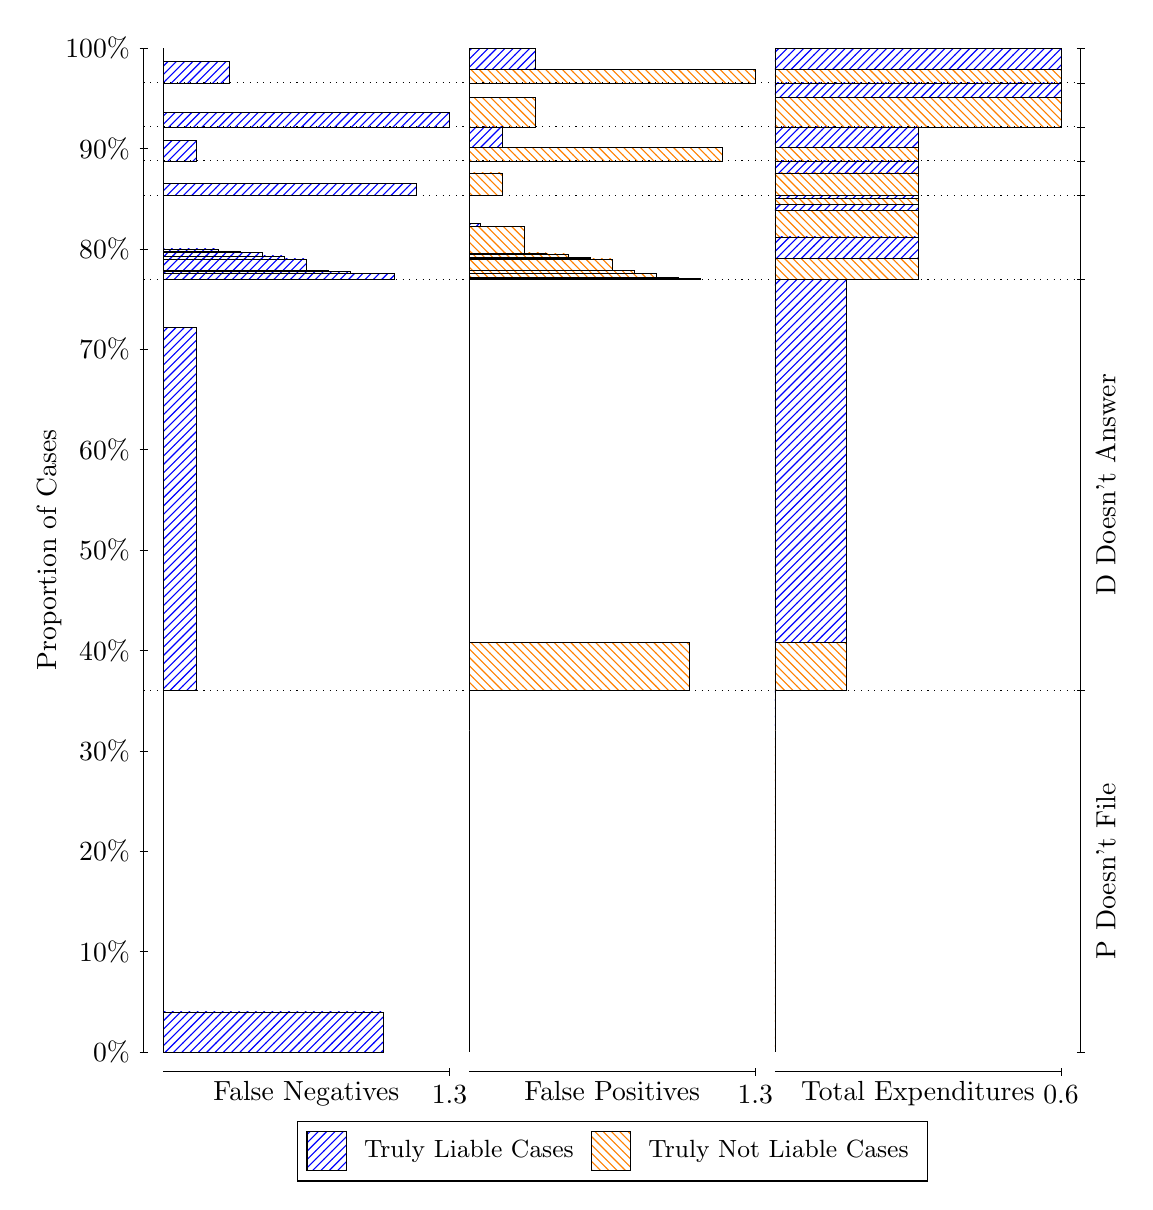
\begin{tikzpicture}
\draw[black, very thin] (1.5,1.75) -- (1.5,14.5);
\node[rotate=90, anchor=center] at (0.3, 8.125) {Proportion of Cases};
\draw[black, very thin] (1.45,1.75) -- (1.55,1.75);
\node[anchor=east] at (1.45, 1.75) {0\%};
\draw[black, very thin] (1.45,3.025) -- (1.55,3.025);
\node[anchor=east] at (1.45, 3.025) {10\%};
\draw[black, very thin] (1.45,4.3) -- (1.55,4.3);
\node[anchor=east] at (1.45, 4.3) {20\%};
\draw[black, very thin] (1.45,5.575) -- (1.55,5.575);
\node[anchor=east] at (1.45, 5.575) {30\%};
\draw[black, very thin] (1.45,6.85) -- (1.55,6.85);
\node[anchor=east] at (1.45, 6.85) {40\%};
\draw[black, very thin] (1.45,8.125) -- (1.55,8.125);
\node[anchor=east] at (1.45, 8.125) {50\%};
\draw[black, very thin] (1.45,9.4) -- (1.55,9.4);
\node[anchor=east] at (1.45, 9.4) {60\%};
\draw[black, very thin] (1.45,10.675) -- (1.55,10.675);
\node[anchor=east] at (1.45, 10.675) {70\%};
\draw[black, very thin] (1.45,11.95) -- (1.55,11.95);
\node[anchor=east] at (1.45, 11.95) {80\%};
\draw[black, very thin] (1.45,13.225) -- (1.55,13.225);
\node[anchor=east] at (1.45, 13.225) {90\%};
\draw[black, very thin] (1.45,14.5) -- (1.55,14.5);
\node[anchor=east] at (1.45, 14.5) {100\%};

\draw[black, very thin] (13.4,1.75) -- (13.4,14.5);
\draw[black, very thin] (13.35,1.75) -- (13.45,1.75);
\node[anchor=west] at (13.35, 1.75) {};
\draw[black, very thin] (13.35,6.3442) -- (13.45,6.3442);
\node[anchor=west] at (13.35, 6.3442) {};
\draw[black, very thin] (13.35,11.56) -- (13.45,11.56);
\node[anchor=west] at (13.35, 11.56) {};
\draw[black, very thin] (13.35,12.628) -- (13.45,12.628);
\node[anchor=west] at (13.35, 12.628) {};
\draw[black, very thin] (13.35,13.066) -- (13.45,13.066);
\node[anchor=west] at (13.35, 13.066) {};
\draw[black, very thin] (13.35,13.498) -- (13.45,13.498);
\node[anchor=west] at (13.35, 13.498) {};
\draw[black, very thin] (13.35,14.058) -- (13.45,14.058);
\node[anchor=west] at (13.35, 14.058) {};
\draw[black, very thin] (13.35,14.5) -- (13.45,14.5);
\node[anchor=west] at (13.35, 14.5) {};

\draw[black, very thin, pattern color=blue, pattern=north east lines] (1.75,1.75) rectangle (4.5449,2.2585);
\draw[black, very thin, pattern color=orange, pattern=north west lines] (1.75,2.2585) rectangle (1.75,6.3442);
\draw[black, very thin, pattern color=blue, pattern=north east lines] (1.75,6.3442) rectangle (2.1692,10.95);
\draw[black, very thin, pattern color=orange, pattern=north west lines] (1.75,10.95) rectangle (1.75,11.56);
\draw[black, very thin, pattern color=blue, pattern=north east lines] (1.75,11.56) rectangle (4.6846,11.634);
\draw[black, very thin, pattern color=blue, pattern=north east lines] (1.75,11.634) rectangle (4.4051,11.638);
\draw[black, very thin, pattern color=blue, pattern=north east lines] (1.75,11.638) rectangle (4.1256,11.667);
\draw[black, very thin, pattern color=blue, pattern=north east lines] (1.75,11.667) rectangle (3.8462,11.679);
\draw[black, very thin, pattern color=blue, pattern=north east lines] (1.75,11.679) rectangle (3.5667,11.821);
\draw[black, very thin, pattern color=blue, pattern=north east lines] (1.75,11.821) rectangle (3.2872,11.86);
\draw[black, very thin, pattern color=blue, pattern=north east lines] (1.75,11.86) rectangle (3.0077,11.904);
\draw[black, very thin, pattern color=blue, pattern=north east lines] (1.75,11.904) rectangle (2.7282,11.917);
\draw[black, very thin, pattern color=blue, pattern=north east lines] (1.75,11.917) rectangle (2.4487,11.95);
\draw[black, very thin, pattern color=orange, pattern=north west lines] (1.75,11.95) rectangle (1.75,12.628);
\draw[black, very thin, pattern color=blue, pattern=north east lines] (1.75,12.628) rectangle (4.9641,12.78);
\draw[black, very thin, pattern color=orange, pattern=north west lines] (1.75,12.78) rectangle (1.75,13.066);
\draw[black, very thin, pattern color=blue, pattern=north east lines] (1.75,13.066) rectangle (2.1692,13.328);
\draw[black, very thin, pattern color=orange, pattern=north west lines] (1.75,13.328) rectangle (1.75,13.498);
\draw[black, very thin, pattern color=blue, pattern=north east lines] (1.75,13.498) rectangle (5.3833,13.679);
\draw[black, very thin, pattern color=orange, pattern=north west lines] (1.75,13.679) rectangle (1.75,14.058);
\draw[black, very thin, pattern color=blue, pattern=north east lines] (1.75,14.058) rectangle (2.5885,14.334);
\draw[black, very thin, pattern color=orange, pattern=north west lines] (1.75,14.334) rectangle (1.75,14.5);
\draw[black, very thin, pattern color=orange, pattern=north west lines] (5.6333,1.75) rectangle (5.6333,5.8357);
\draw[black, very thin, pattern color=blue, pattern=north east lines] (5.6333,5.8357) rectangle (5.6333,6.3442);
\draw[black, very thin, pattern color=orange, pattern=north west lines] (5.6333,6.3442) rectangle (8.4282,6.955);
\draw[black, very thin, pattern color=blue, pattern=north east lines] (5.6333,6.955) rectangle (5.6333,11.56);
\draw[black, very thin, pattern color=orange, pattern=north west lines] (5.6333,11.56) rectangle (8.5679,11.579);
\draw[black, very thin, pattern color=orange, pattern=north west lines] (5.6333,11.579) rectangle (8.2885,11.592);
\draw[black, very thin, pattern color=orange, pattern=north west lines] (5.6333,11.592) rectangle (8.009,11.636);
\draw[black, very thin, pattern color=orange, pattern=north west lines] (5.6333,11.636) rectangle (7.7295,11.675);
\draw[black, very thin, pattern color=orange, pattern=north west lines] (5.6333,11.675) rectangle (7.45,11.822);
\draw[black, very thin, pattern color=orange, pattern=north west lines] (5.6333,11.822) rectangle (7.1705,11.827);
\draw[black, very thin, pattern color=orange, pattern=north west lines] (5.6333,11.827) rectangle (7.1705,11.84);
\draw[black, very thin, pattern color=orange, pattern=north west lines] (5.6333,11.84) rectangle (6.891,11.886);
\draw[black, very thin, pattern color=orange, pattern=north west lines] (5.6333,11.886) rectangle (6.6115,11.898);
\draw[black, very thin, pattern color=orange, pattern=north west lines] (5.6333,11.898) rectangle (6.3321,12.238);
\draw[black, very thin, pattern color=blue, pattern=north east lines] (5.6333,12.238) rectangle (5.7731,12.271);
\draw[black, very thin, pattern color=blue, pattern=north east lines] (5.6333,12.271) rectangle (5.6333,12.628);
\draw[black, very thin, pattern color=orange, pattern=north west lines] (5.6333,12.628) rectangle (6.0526,12.914);
\draw[black, very thin, pattern color=blue, pattern=north east lines] (5.6333,12.914) rectangle (5.6333,13.066);
\draw[black, very thin, pattern color=orange, pattern=north west lines] (5.6333,13.066) rectangle (8.8474,13.236);
\draw[black, very thin, pattern color=blue, pattern=north east lines] (5.6333,13.236) rectangle (6.0526,13.498);
\draw[black, very thin, pattern color=orange, pattern=north west lines] (5.6333,13.498) rectangle (6.4718,13.877);
\draw[black, very thin, pattern color=blue, pattern=north east lines] (5.6333,13.877) rectangle (5.6333,14.058);
\draw[black, very thin, pattern color=orange, pattern=north west lines] (5.6333,14.058) rectangle (9.2667,14.224);
\draw[black, very thin, pattern color=blue, pattern=north east lines] (5.6333,14.224) rectangle (6.4718,14.5);
\draw[black, very thin, pattern color=orange, pattern=north west lines] (9.5167,1.75) rectangle (9.5167,5.8357);
\draw[black, very thin, pattern color=blue, pattern=north east lines] (9.5167,5.8357) rectangle (9.5167,6.3442);
\draw[black, very thin, pattern color=orange, pattern=north west lines] (9.5167,6.3442) rectangle (10.425,6.955);
\draw[black, very thin, pattern color=blue, pattern=north east lines] (9.5167,6.955) rectangle (10.425,11.56);
\draw[black, very thin, pattern color=orange, pattern=north west lines] (9.5167,11.56) rectangle (11.333,11.827);
\draw[black, very thin, pattern color=blue, pattern=north east lines] (9.5167,11.827) rectangle (11.333,12.102);
\draw[black, very thin, pattern color=orange, pattern=north west lines] (9.5167,12.102) rectangle (11.333,12.442);
\draw[black, very thin, pattern color=blue, pattern=north east lines] (9.5167,12.442) rectangle (11.333,12.516);
\draw[black, very thin, pattern color=orange, pattern=north west lines] (9.5167,12.516) rectangle (11.333,12.586);
\draw[black, very thin, pattern color=blue, pattern=north east lines] (9.5167,12.586) rectangle (11.333,12.628);
\draw[black, very thin, pattern color=orange, pattern=north west lines] (9.5167,12.628) rectangle (11.333,12.914);
\draw[black, very thin, pattern color=blue, pattern=north east lines] (9.5167,12.914) rectangle (11.333,13.066);
\draw[black, very thin, pattern color=orange, pattern=north west lines] (9.5167,13.066) rectangle (11.333,13.236);
\draw[black, very thin, pattern color=blue, pattern=north east lines] (9.5167,13.236) rectangle (11.333,13.498);
\draw[black, very thin, pattern color=orange, pattern=north west lines] (9.5167,13.498) rectangle (13.15,13.877);
\draw[black, very thin, pattern color=blue, pattern=north east lines] (9.5167,13.877) rectangle (13.15,14.058);
\draw[black, very thin, pattern color=orange, pattern=north west lines] (9.5167,14.058) rectangle (13.15,14.224);
\draw[black, very thin, pattern color=blue, pattern=north east lines] (9.5167,14.224) rectangle (13.15,14.5);
\draw[black, dotted] (1.5,6.3442) -- (13.4,6.3442);
\draw[black, dotted] (1.5,11.56) -- (13.4,11.56);
\draw[black, dotted] (1.5,12.628) -- (13.4,12.628);
\draw[black, dotted] (1.5,13.066) -- (13.4,13.066);
\draw[black, dotted] (1.5,13.498) -- (13.4,13.498);
\draw[black, dotted] (1.5,14.058) -- (13.4,14.058);
\draw[black, very thin] (1.75,1.5) -- (5.3833,1.5);
\node[anchor=north] at (3.5667, 1.5) {False Negatives};
\draw[black, very thin] (5.3833,1.45) -- (5.3833,1.55);
\node[anchor=north] at (5.3833, 1.45) {1.3};

\draw[black, very thin] (5.6333,1.5) -- (9.2667,1.5);
\node[anchor=north] at (7.45, 1.5) {False Positives};
\draw[black, very thin] (9.2667,1.45) -- (9.2667,1.55);
\node[anchor=north] at (9.2667, 1.45) {1.3};

\draw[black, very thin] (9.5167,1.5) -- (13.15,1.5);
\node[anchor=north] at (11.333, 1.5) {Total Expenditures};
\draw[black, very thin] (13.15,1.45) -- (13.15,1.55);
\node[anchor=north] at (13.15, 1.45) {0.6};

\node[black, centered, rotate=90] at (13.72, 4.0471) {P Doesn't File};
\node[black, centered, rotate=90] at (13.72, 8.9523) {D Doesn't Answer};






\draw (7.449999999999999,1.5) node[draw=none] (baseCoordinate) {};
\begin{scope}[align=center]
        \matrix[scale=0.5, draw=black, below=0.5cm of baseCoordinate, nodes={draw}, column sep=0.1cm]{
            \node[rectangle, draw, minimum width=0.5cm, minimum height=0.5cm, pattern=north east lines, pattern color=blue] {}; &
            \node[draw=none, font=\small] (B) {Truly Liable Cases}; &
            \node[rectangle, draw, minimum width=0.5cm, minimum height=0.5cm, pattern=north west lines, pattern color=orange] {}; &
            \node[draw=none, font=\small] (B) {Truly Not Liable Cases}; \\
            };
\end{scope}

\end{tikzpicture}
\end{document}